\section{Алгоритм с заметающей прямой}


\begin{frame}{Постановка задачи}
    Дано множество отрезков на плоскости,\\
    найти всевозможные их пересечения $\{x_i\}$\\
    и вместе с каждой точкой $x_i$ --- множество отрезков,\\
    пересекающихся в ней.
\end{frame}

%\begin{frame}{}
        %Если отрезки имеют общую точку то, когда их проекции на ось ординат имеют общую точку. Поэтому будем искать пересечения среди пар отрезков, пересекающих одну и ту же горизонтальную прямую. \\
	%\vspace{-1mm}
%\end{frame}

\begin{frame}{Заметающая прямая}
        Запустим горизонтальную {\it sweep line}, начинающую\\
        свое движение {\it над всеми} отрезками входа.\\
        (Разумеется, мы не будем реализовывать
        {\it непрерывное} движение)
        \vspace{-7mm}
        
        \begin{center}
        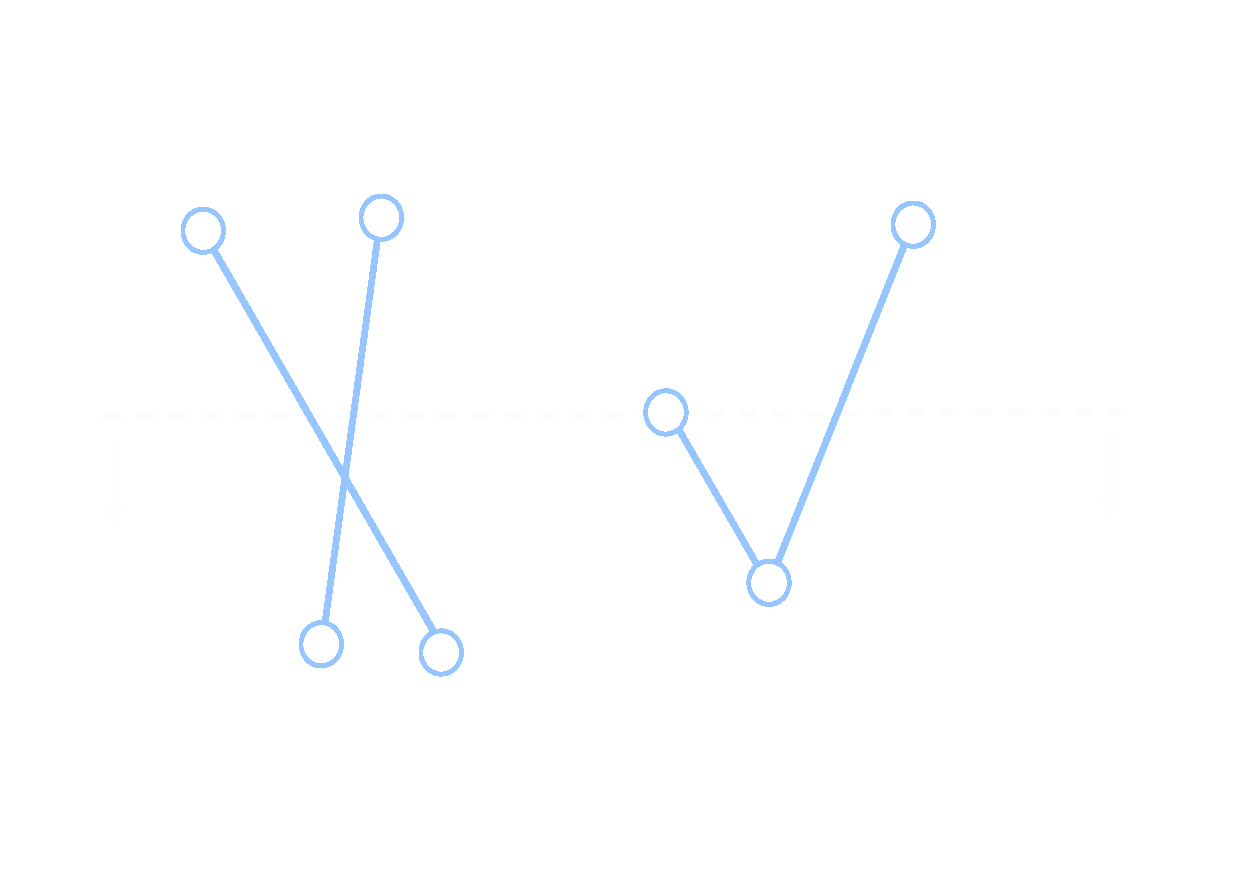
\includegraphics[width=0.6\textwidth]{картинки/нормкартинки/sweepline1.pdf}
	\end{center}
\end{frame}

\begin{frame}{Event points}
        Вершины, соответствующие концам отрезков,\\
        будем называть {\it крайними событиями,}\\
        а их пересечениям~— {\it внутренними событиями.}\\
        Упорядочим события следующим образом:
        \[ p \prec q\ \ \longleftrightarrow\ \ \left[ 
      \begin{gathered} 
        p_y > q_y \\ 
        p_y = q_y, \; p_x < q_x \\ 
      \end{gathered} 
       \right. \]
\end{frame}


\begin{frame}{Статус}
        \vphantom{x}{\it Статусом заметающей прямой} будем называть\\
        последовательность отрезков, пересекающих её\\
        в данный момент.

        \begin{center}
        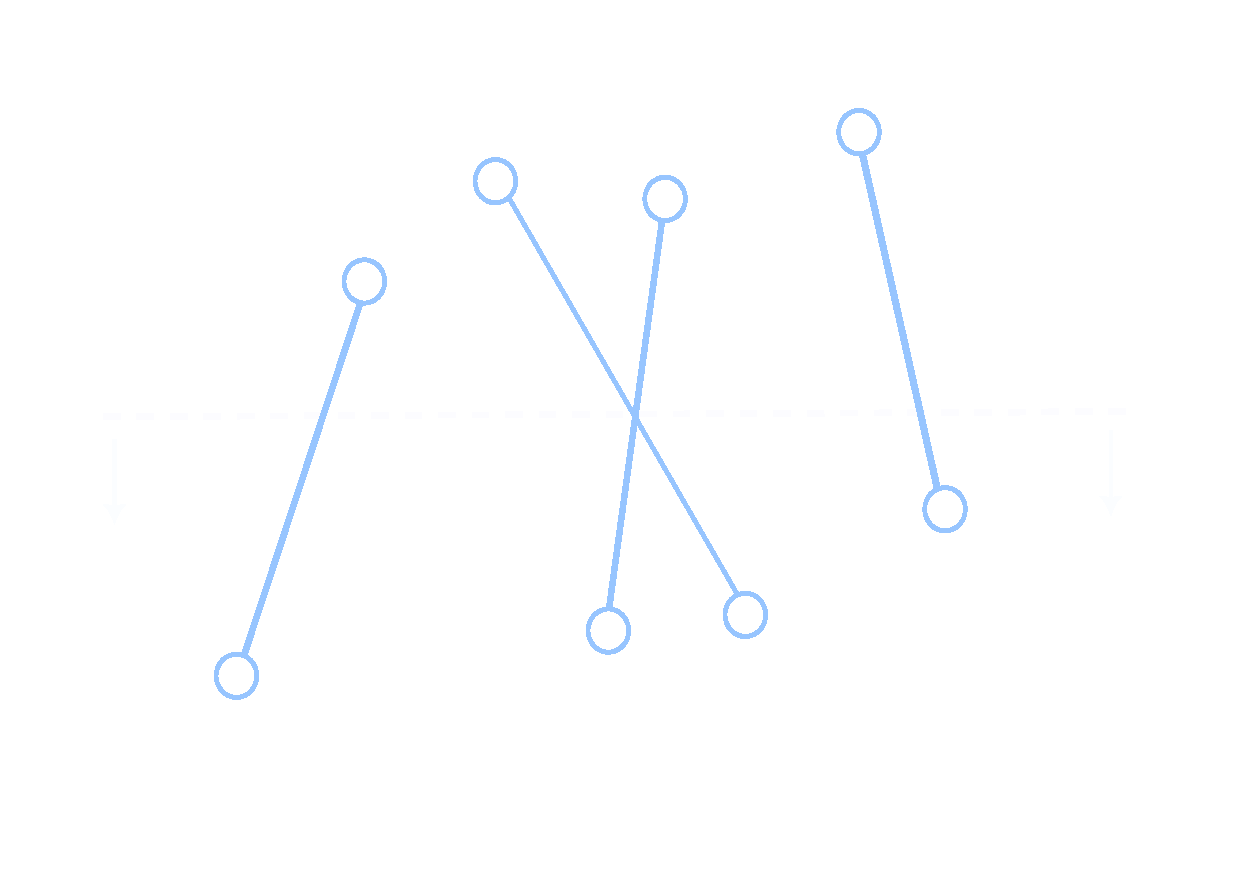
\includegraphics[width=0.5\textwidth]{картинки/нормкартинки/sweepline2.pdf}
	\end{center}
\end{frame}

\begin{frame}{Статус}
        \vphantom{x}{\it Статусом заметающей прямой} будем называть\\
        последовательность отрезков, пересекающих её\\
        в данный момент.

        \begin{center}
        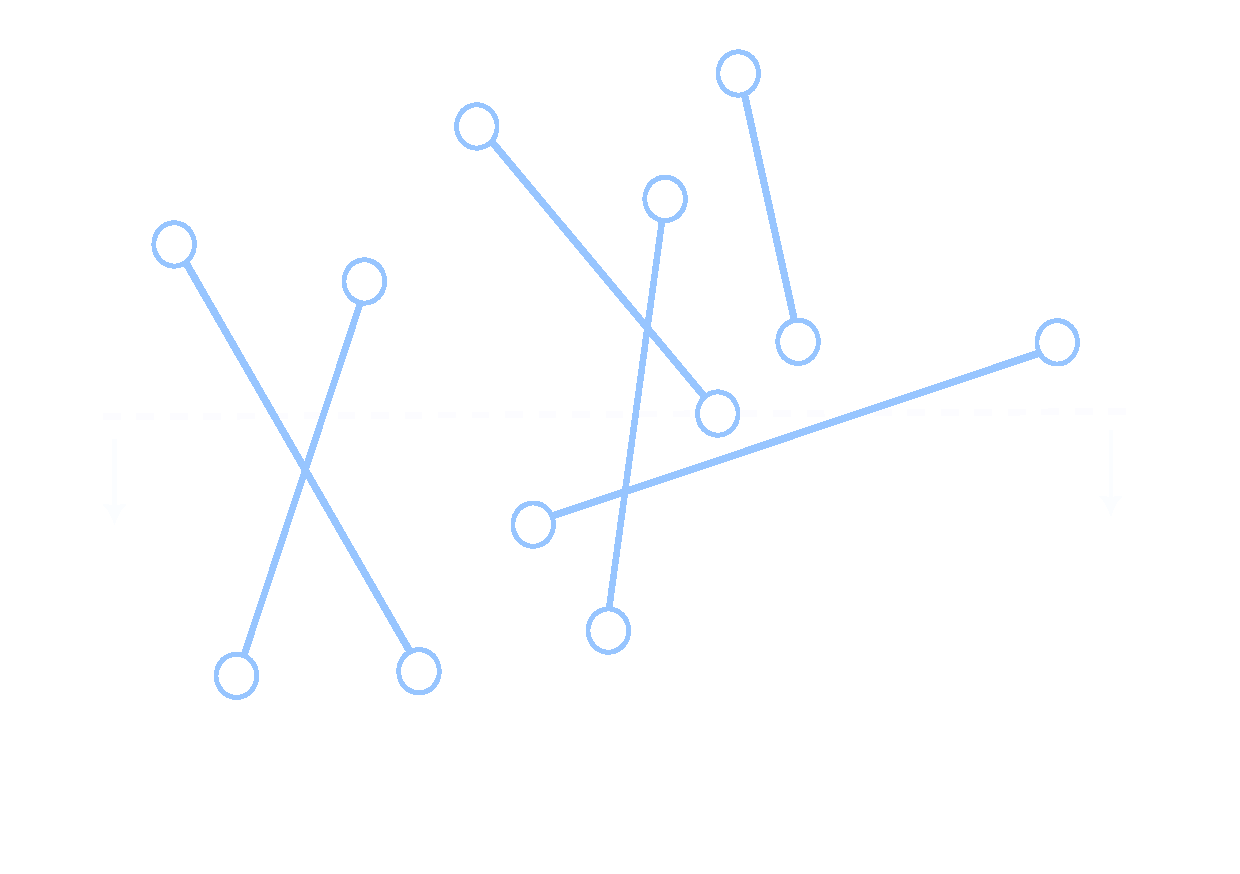
\includegraphics[width=0.5\textwidth]{картинки/нормкартинки/sweepline3.pdf}
	\end{center}
\end{frame}

\begin{frame}{Бинарное дерево статуса}
        Для хранения статуса используем бинарное дерево $T$. Оно\\ понадобится нам для нахождения ближайших к событию отрезков.

    \begin{center}
        \includegraphics[width=0.43\textwidth]%
          {картинки/нормкартинки/sweepline_for_tree.pdf}
        \ \ 
        \includegraphics[width=0.43\textwidth]%
          {картинки/нормкартинки/tree.pdf} 
    \end{center}
\end{frame}

\begin{frame}{Общий алгоритм}
        \begin{itemize}
            \item создаем пустую очередь $Q$ и заполняем ее\\
            крайними событиями (если событие --- верхняя вершина\\
            отрезка $s$, то кладем $s$ вместе с ней) 
            \item создаем пустое дерево статуса
            \item пока $Q \neq \varnothing$, определяем,
            какое событие будет следующим,\\
            удаляем текущее и обрабатываем следующее 
        \end{itemize}
\end{frame}

\begin{frame}{Обработка события}
    $U(p)$ --- отрезки, верхняя вершина которых $p$ \\ %см очередь, там они есть
    $L(p)$ --- отрезки, нижняя вершина которых $p$ \\
    $C(p)$ --- отрезки, содержащие $p$ внутри \medskip \\

 \begin{algorithmic}
    \If{$U(p) \cup L(p) \cup C(p) \neq \varnothing$}
        \State $p$ --- пересечение набора отрезков $U(p) \cup L(p) \cup C(p)$
    \EndIf
    \State удаляем отрезки из $L(p) \cup C(p)$
    \State добавляем отрезки из $U(p) \cup C(p)$
 \end{algorithmic}
\end{frame}

\begin{frame}{Обработка события}
 \begin{algorithmic}
    \If{$U(p) \cup C(p) = \varnothing$}
        \State находим соседей $p$ с помощью $T$ --- $s_l$, $s_r$
        \State $\text{FindNewEvent}\lr*{s_l,s_r,p}$
    \Else 
        \State $s' \coloneqq$ крайний левый в $U(p) \cup C(p)$
        \State $s_l \coloneqq$ слева от $s^{\prime}$
        \State $\text{FindNewEvent}\lr*{s_l,s^{\prime},p}$
        \State $s^{\prime\prime} \coloneqq$ крайний правый в $U(p) \cup C(p)$
        \State $s_r \coloneqq$ справа от $s^{\prime\prime}$
        \State $\text{FindNewEvent}\lr*{s^{\prime\prime},s_r,p}$
    \EndIf
\end{algorithmic} 
\end{frame}

\begin{frame}{Сложность}
    $O\lr*{n \cdot \log n}$ --- заполнение очереди

    Пока $Q \neq \varnothing$ ($\leq 2n+I$ раз) \\
    \qquad изменение очереди~— $O(\log n)$ \\
    \qquad изменение дерева статуса~—
        $O\lr*{\log n \cdot \left|U(p) \cup L(p) \cup C(p)\right|}$
        \vspace{-6mm}

   \[ \sum\limits_{p}|U(p) \cup L(p) \cup C(p)|\ \ =\ \ O(2n+I)\ \ =\ \ O(n+I) \]
   \vspace{-16mm}

  \begin{multline*}
     O\lr*{n \cdot \log n} + O\lr*{\lr*{2n+I} \cdot \log n} +
       O\lr*{\log n \cdot \sum\limits_{p}|U(p) \cup L(p) \cup C(p)|} = \\
       = O\lr*{\lr*{n+I}\cdot \log n}
  \end{multline*}
\end{frame}
